\documentclass[a4paper]{article}
\usepackage[a4paper,landscape,margin=12mm]{geometry}
\usepackage[T1]{fontenc}
\usepackage{lmodern}
\usepackage{tikz}
\usetikzlibrary{arrows.meta,positioning,fit}
\pagestyle{empty}
\setlength{\parindent}{0pt}
\begin{document}
\begin{center}
{\large\bfseries [week-08] 26512071 -- fair-furniture: Round 3 agent architecture (snapshot 2026-11-17 17:55 KST)}
\end{center}
\vspace{-1mm}
\begin{center}
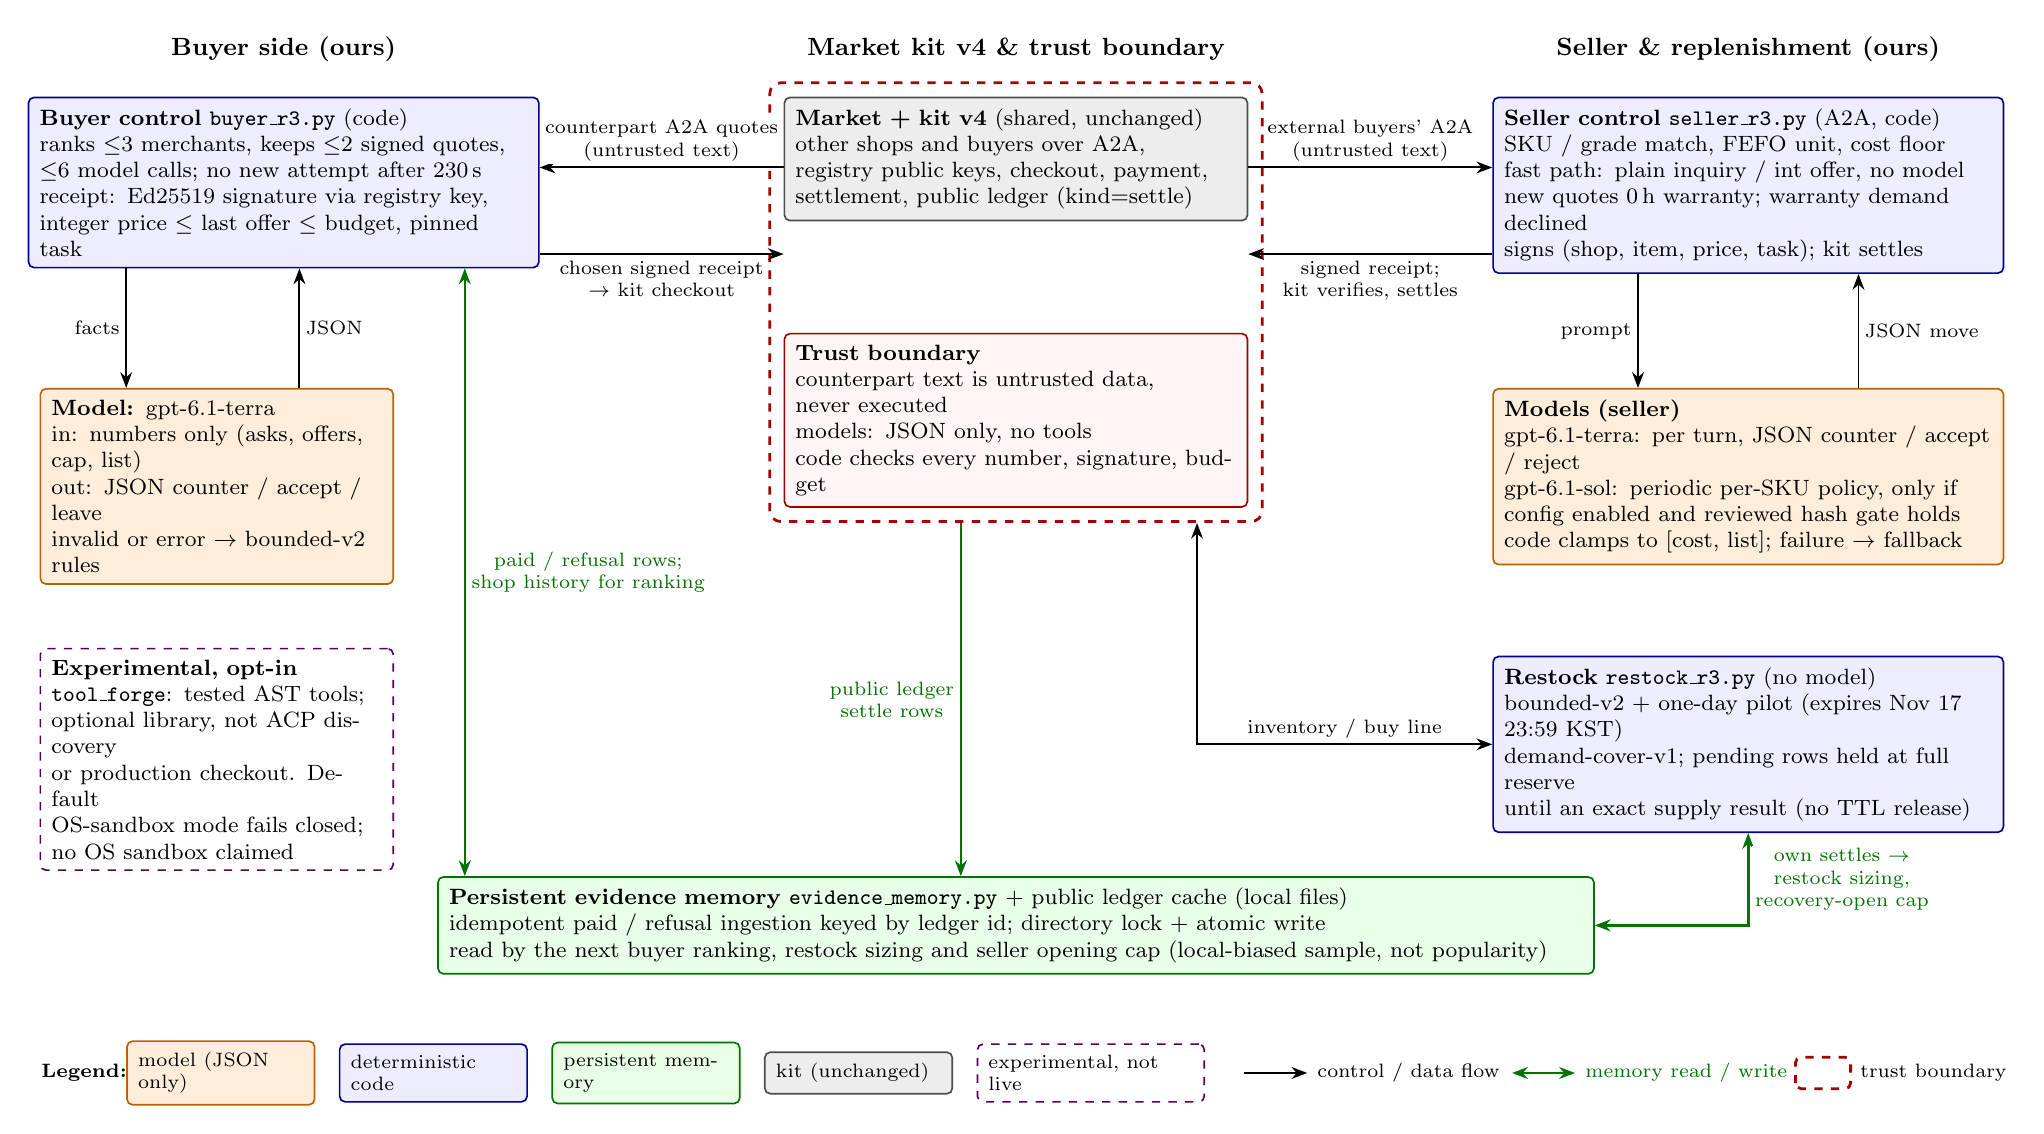
\begin{tikzpicture}[
  font=\footnotesize,
  box/.style={draw, rounded corners=2pt, align=left, text width=#1, inner sep=4pt, line width=0.6pt},
  ctl/.style={box=#1, fill=blue!7, draw=blue!60!black},
  mdl/.style={box=#1, fill=orange!14, draw=orange!75!black},
  mem/.style={box=#1, fill=green!9, draw=green!45!black},
  kitbox/.style={box=#1, fill=gray!14, draw=gray!60!black},
  xpr/.style={box=#1, dashed, fill=white, draw=violet!70!black},
  flow/.style={-{Stealth[length=2mm]}, line width=0.7pt},
  bidir/.style={{Stealth[length=2mm]}-{Stealth[length=2mm]}, line width=0.7pt},
  memf/.style={{Stealth[length=2mm]}-{Stealth[length=2mm]}, line width=0.9pt, green!45!black},
  memo/.style={-{Stealth[length=2mm]}, line width=0.9pt, green!45!black},
  lab/.style={font=\scriptsize, fill=white, inner sep=1pt, align=center},
  head/.style={font=\small\bfseries}
]
% column headers
\node[head] at (3.4,0) {Buyer side (ours)};
\node[head] at (12.7,0) {Market kit v4 \& trust boundary};
\node[head] at (22.0,0) {Seller \& replenishment (ours)};

% buyer column
\node[ctl=6.2cm, anchor=north] (A) at (3.4,-0.6) {\textbf{Buyer control} \texttt{buyer\_r3.py} (code)\\
 ranks $\le$3 merchants, keeps $\le$2 signed quotes,\\
 $\le$6 model calls; no new attempt after 230\,s\\
 receipt: Ed25519 signature via registry key,\\
 integer price $\le$ last offer $\le$ budget, pinned task};
\node[mdl=4.2cm, anchor=north west] (B) at (0.3,-4.3) {\textbf{Model:} gpt-6.1-terra\\
 in: numbers only (asks, offers, cap, list)\\
 out: JSON counter / accept / leave\\
 invalid or error $\rightarrow$ bounded-v2 rules};
\node[xpr=4.2cm, anchor=north west] (H) at (0.3,-7.6) {\textbf{Experimental, opt-in}\\
 \texttt{tool\_forge}: tested AST tools;\\
 optional library, not ACP discovery\\
 or production checkout. Default\\
 OS-sandbox mode fails closed;\\
 no OS sandbox claimed};

% kit column
\node[kitbox=5.6cm, anchor=north] (C) at (12.7,-0.6) {\textbf{Market + kit v4} (shared, unchanged)\\
 other shops and buyers over A2A,\\
 registry public keys, checkout, payment,\\
 settlement, public ledger (kind=settle)};
\node[box=5.6cm, anchor=north, fill=red!4, draw=red!60!black] (T) at (12.7,-3.6) {\textbf{Trust boundary}\\
 counterpart text is untrusted data,\\ never executed\\
 models: JSON only, no tools\\
 code checks every number, signature, budget};
\node[draw=red!65!black, dashed, line width=1pt, rounded corners=4pt, inner sep=5pt, fit=(C)(T)] (TB) {};

% seller column
\node[ctl=6.2cm, anchor=north] (D) at (22.0,-0.6) {\textbf{Seller control} \texttt{seller\_r3.py} (A2A, code)\\
 SKU / grade match, FEFO unit, cost floor\\
 fast path: plain inquiry / int offer, no model\\
 new quotes 0\,h warranty; warranty demand declined\\
 signs (shop, item, price, task); kit settles};
\node[mdl=6.2cm, anchor=north] (E) at (22.0,-4.3) {\textbf{Models (seller)}\\
 gpt-6.1-terra: per turn, JSON counter / accept / reject\\
 gpt-6.1-sol: periodic per-SKU policy, only if\\
 config enabled and reviewed hash gate holds\\
 code clamps to [cost, list]; failure $\rightarrow$ fallback};
\node[ctl=6.2cm, anchor=north] (F) at (22.0,-7.7) {\textbf{Restock} \texttt{restock\_r3.py} (no model)\\
 bounded-v2 + one-day pilot (expires Nov 17 23:59 KST)\\
 demand-cover-v1; pending rows held at full reserve\\
 until an exact supply result (no TTL release)};

% memory
\node[mem=14.4cm, anchor=north] (G) at (12.7,-10.5) {\textbf{Persistent evidence memory} \texttt{evidence\_memory.py} + public ledger cache (local files)\\
 idempotent paid / refusal ingestion keyed by ledger id; directory lock + atomic write\\
 read by the next buyer ranking, restock sizing and seller opening cap (local-biased sample, not popularity)};

% helper coordinates
\coordinate (r1) at (0,-1.5);
\coordinate (r2) at (0,-2.6);
\coordinate (bx1) at (1.4,0);
\coordinate (bx2) at (3.6,0);
\coordinate (dx1) at (20.6,0);
\coordinate (dx2) at (23.4,0);
\coordinate (kx) at (15.0,0);
\coordinate (mx) at (12.0,0);
\coordinate (ax) at (5.7,0);

% buyer <-> market
\draw[flow] (C.west |- r1) -- node[lab, above=1pt] {counterpart A2A quotes\\(untrusted text)} (A.east |- r1);
\draw[flow] (A.east |- r2) -- node[lab, below=1pt] {chosen signed receipt\\$\rightarrow$ kit checkout} (C.west |- r2);
% market <-> seller
\draw[flow] (C.east |- r1) -- node[lab, above=1pt] {external buyers' A2A\\(untrusted text)} (D.west |- r1);
\draw[flow] (D.west |- r2) -- node[lab, below=1pt] {signed receipt;\\kit verifies, settles} (C.east |- r2);
% control <-> model
\draw[flow] (A.south -| bx1) -- node[lab, left=1pt] {facts} (B.north -| bx1);
\draw[flow] (B.north -| bx2) -- node[lab, right=1pt] {JSON} (A.south -| bx2);
\draw[flow] (D.south -| dx1) -- node[lab, left=1pt] {prompt} (E.north -| dx1);
\draw[flow] (E.north -| dx2) -- node[lab, right=1pt] {JSON move} (D.south -| dx2);
% kit <-> restock
\draw[bidir] (TB.south -| kx) |- node[lab, pos=0.75, above=1pt] {inventory / buy line} (F.west);
% memory feedback
\draw[memo] (TB.south -| mx) -- node[lab, left=1pt] {public ledger\\settle rows} (G.north -| mx);
\draw[memf] (A.south -| ax) -- node[lab, right=1pt] {paid / refusal rows;\\shop history for ranking} (G.north -| ax);
\draw[memf] (G.east) -| node[lab, pos=0.75, right=1pt] {own settles $\rightarrow$\\restock sizing,\\recovery-open cap} (F.south);

% legend
\node[anchor=west, font=\scriptsize\bfseries] at (0.2,-13.0) {Legend:};
\node[mdl=2.1cm, font=\scriptsize, anchor=west] at (1.4,-13.0) {model (JSON only)};
\node[ctl=2.1cm, font=\scriptsize, anchor=west] at (4.1,-13.0) {deterministic code};
\node[mem=2.1cm, font=\scriptsize, anchor=west] at (6.8,-13.0) {persistent memory};
\node[kitbox=2.1cm, font=\scriptsize, anchor=west] at (9.5,-13.0) {kit (unchanged)};
\node[xpr=2.6cm, font=\scriptsize, anchor=west] at (12.2,-13.0) {experimental, not live};
\draw[flow] (15.6,-13.0) -- ++(0.8,0) node[right, font=\scriptsize] {control / data flow};
\draw[memf] (19.0,-13.0) -- ++(0.8,0) node[right, font=\scriptsize] {memory read / write};
\draw[draw=red!65!black, dashed, line width=1pt, rounded corners=2pt] (22.6,-13.2) rectangle ++(0.7,0.4);
\node[right, font=\scriptsize] at (23.3,-13.0) {trust boundary};
\end{tikzpicture}
\end{center}
\vspace{1mm}
\parbox{\linewidth}{\footnotesize\textbf{Figure.} Original design versus kit: shared kit v4 (grey) handles registered public keys, checkout, payment and settlement unchanged. Our control, models and memory close an outcome-to-next-decision loop: numeric-only buyer context and two verified quote candidates; guarded Terra negotiation, gated periodic Sol policy and an own-12h paid-price opening cap (a mixed-condition heuristic, not matched comparables); model-free replenishment with durable UNKNOWN liabilities. Amendment 8 disables simulated financial caps but retains expiry and historical obligations; new 0h warranties do not erase 64 issued authorities. Models have no executable tools. The optional \texttt{tool\_forge} source is included but not on the live checkout route; the durable-checkout candidate is neither included nor deployed. Runtime evidence and limitations are separate in REPORT.md.}
\end{document}
